% This file is a solution template for:
% \usepackage{pgfpages}
% \pgfpagesuselayout{2 on 1}[a4paper,border shrink=5mm]
%\usepackage[spanish]{babel}
% for \mathds{N}
%\newtheorem{assumption_1}{Assumption 1: Firms Maximize Profits}
%\newtheorem{assumption_2}{Assumption 2: Firms are Right on Average}
%\newtheorem{assumption_3}{Assumption 3: Orthogonality}
% or ...
% \setbeamercovered{transparent}
% or whatever (possibly just delete it)
%\beamerdefaultoverlayspecification{<+->}
%\hypersetup{colorlinks=true,linkcolor=red}


\documentclass[10pt,letterpaper]{beamer}
%%%%%%%%%%%%%%%%%%%%%%%%%%%%%%%%%%%%%%%%%%%%%%%%%%%%%%%%%%%%%%%%%%%%%%%%%%%%%%%%%%%%%%%%%%%%%%%%%%%%%%%%%%%%%%%%%%%%%%%%%%%%%%%%%%%%%%%%%%%%%%%%%%%%%%%%%%%%%%%%%%%%%%%%%%%%%%%%%%%%%%%%%%%%%%%%%%%%%%%%%%%%%%%%%%%%%%%%%%%%%%%%%%%%%%%%%%%%%%%%%%%%%%%%%%%%
\usepackage{graphicx}
\usepackage[latin1]{inputenc}
\usepackage{listings}
\usepackage{amsmath}
\usepackage{amsfonts}
\usepackage{amsxtra}
\usepackage{amstext}
\usepackage{amssymb}
\usepackage{latexsym}
\usepackage{subfigure}
\usepackage{eurosym}
\usepackage{multimedia}
\usepackage{dsfont}
\usepackage{graphicx}
\usepackage{color,colortbl}
\usepackage{multirow}
\usepackage{bbm}

\setcounter{MaxMatrixCols}{10}
%TCIDATA{OutputFilter=Latex.dll}
%TCIDATA{Version=5.50.0.2890}
%TCIDATA{<META NAME="SaveForMode" CONTENT="1">}
%TCIDATA{BibliographyScheme=Manual}
%TCIDATA{LastRevised=Tuesday, March 04, 2014 20:30:42}
%TCIDATA{<META NAME="GraphicsSave" CONTENT="32">}

\linespread{1.2}
\definecolor{clearBlue}{cmyk}{0.15,0.1,0,0.1}
\newcommand{\bluecell}{\cellcolor{clearBlue}}
\newtheorem{assumption}{Assumption}
\newcommand{\argmax}{\operatornamewithlimits{argmax}}
\newcommand{\argmin}{\operatornamewithlimits{argmin}}
\mode<presentation> {
  \usetheme{Singapore}
  
 
  
  \setbeamertemplate{navigation symbols}{}
}
\defbeamertemplate*{footline}{my theme}
{
  \leavevmode
  \hbox{  \begin{beamercolorbox}[wd=.333333\paperwidth,ht=2.25ex,dp=1ex,center]{author in head/foot}    \usebeamerfont{author in head/foot}\insertshortauthor~~(\insertshortinstitute)
  \end{beamercolorbox}  \begin{beamercolorbox}[wd=.333333\paperwidth,ht=2.25ex,dp=1ex,center]{title in head/foot}    \usebeamerfont{title in head/foot}\insertshorttitle
  \end{beamercolorbox}  \begin{beamercolorbox}[wd=.333333\paperwidth,ht=2.25ex,dp=1ex,right]{date in head/foot}    \usebeamerfont{date in head/foot}\insertshortdate{}\hspace*{2em}
  \end{beamercolorbox}}
  \vskip0pt
}

%\input{tcilatex}

\begin{document}

\title[Moment Inequalities]{Moment Inequalities - Theory and Applications\\
Dickstein and Morales (2015)}
\author[MJ Dickstein]{Michael J. Dickstein \\
%EndAName
Stanford University}
\institute{Economics 258}

%\date[3/11/13]{March 11, 2013}
%\maketitle
%--------------------------------------------------------------------------------

\begin{frame}
\titlepage
\end{frame}

%--------------------------------------------------------------------------------

\section{Introduction}

%--------------------------------------------------------------------------------

\begin{frame}
\frametitle{{Sources of Error in Empirical Models}\\{Structural Error}}

\begin{itemize}
\item (def'n) components of the agent's payoff function that are known to
the agent but not in the econometrician's dataset

\item typically the single source of error in a structural model

\item Economic theory does not generally place restrictions on its
distribution

\begin{itemize}
\item Econometrician typically chooses the distribution up to a finite
parameter vector 

\item Require independence between structural error and observed covariates
\end{itemize}
\end{itemize}
\end{frame}

%--------------------------------------------------------------------------------

\begin{frame}
\frametitle{{Sources of Error in Empirical Economic Models}\\{Expectational
Error}}

\begin{itemize}
\item (def'n) mismatch between the agent's expectations and the realized
outcome in the future 

\begin{itemize}
\item agent seldom knows the benefits he will earn from deciding to enter a
market, switch jobs, etc 

\item agent forms expectations, and bases his decision on these expectations 
\end{itemize}

\item Why is this a problem?--- econometricians rarely observe measures of
agents ex ante expectations; have only ex post realizations

\item Economic theory---i.e. rational expectations---places restrictions on
this error
\end{itemize}
\end{frame}

%--------------------------------------------------------------------------------

%--------------------------------------------------------------------------------

\begin{frame}
\frametitle{{Sources of Error in Empirical Economic Models}\\{Expectational
Error}}

\begin{itemize}
\item Implication of rational expectations for expectational error: 

\begin{itemize}
\item It is mean independent of the unobserved expectation (analogous to
classical error-in-variables) 

\item It is correlated with the observed covariate 

\item Any variable in the agent's information set is a valid instrumental
variable 
\end{itemize}
\end{itemize}
\end{frame}

%--------------------------------------------------------------------------------

\begin{frame}
\frametitle{Example: Daniel's winery in Chile} \framesubtitle{Daniel's
problem --- export to Venezuela?}

\begin{itemize}
\item Daniel is invited to participate in a wine fair in Caracas, Venezuela
in June 2001. He must decide whether to participate by Dec 31, 2000.

\item Daniel has information on shipping costs and does not face other
export costs

\item Daniel does NOT know the sales revenue he will earn if he attends the
fair

\begin{itemize}
\item forms expectations about export revenues based on market
characteristics 

\item e.g.: past sales revenue of competitors, current political unrest,
nominal exchange rate, etc
\end{itemize}

\item Binary choice: attend fair if expected sales revenue exceed shipping
costs
\end{itemize}
\end{frame}

%--------------------------------------------------------------------------------

\begin{frame}
\frametitle{Example: Daniel's winery in Chile} %
\framesubtitle{Econometrician's problem}

\begin{itemize}
\item Chilean customs agency provides dataset on annual country-specific
sales revenues obtained by each Chilean wine producer during 1995-2005

\item NOT in the data: 

\begin{itemize}
\item Exact shipping cost per mile for Daniel to export to Venezuela 

\item Daniel's expectation as of Dec 31, 2000 about the revenue he might
earn from the fair in 2001 
\end{itemize}
\end{itemize}
\end{frame}

%--------------------------------------------------------------------------------

\begin{frame}
\frametitle{Example: Daniel's winery in Chile} %
\framesubtitle{Econometrician's assumptions: for unobserved shipping costs}

Shipping costs are the \textbf{structural error}

\begin{itemize}
\item They are known to Daniel when he made his export decision, but are not
observed by the econometrician.

\item Assume error is normally distributed around a mean (to estimate); fix
variance to an arbitrary constant.
\end{itemize}
\end{frame}

%-----------------------------------------------------------------------------------

\begin{frame}
\frametitle{Example: Daniel's winery in Chile} %
\framesubtitle{Econometrician's assumptions: for unobserved expectations of
revenue}

Options:

\begin{enumerate}
\item Assume Daniel has perfect foresight. Need: 

\begin{itemize}
\item realized revenues = Daniel's expectations 
\end{itemize}

\item Compute Daniel's unobserved expectations. Need: 

\begin{itemize}
\item Daniel's information set 

\item rational expectations 
\end{itemize}

\item Use ex post measurement of potential revenue as a proxy for the
unobserved expectation. Need: 

\begin{itemize}
\item rational expectations 
\end{itemize}
\end{enumerate}

*** Option 3 imposes fewer assumptions, but introduces error-in-variables
\end{frame}

%--------------------------------------------------------------------------------

\begin{frame}
\frametitle{Goals}

\begin{itemize}
\item Identify and estimate the index coefficients in a binary choice model,
allowing for: 

\begin{enumerate}
\item Individual-specific structural errors 

\item Expectational error (error-in-variables) 
\end{enumerate}

\item Approach: apply moment inequalities
\end{itemize}
\end{frame}

%-----------------------------------------------------------------------------------

\begin{frame}
\frametitle{Outline}

\begin{itemize}
\item Define statistical model

\item Introduce moment inequalities

\item Dickstein and Morales (2015)

\item Inference
\end{itemize}
\end{frame}

%--------------------------------------------------------------------------------

\section{Statistical Model}

%--------------------------------------------------------------------------------
%--------------------------------------------------------------------------------

\begin{frame}
\frametitle{Statistical model} \framesubtitle{Decision rule}

\begin{itemize}
\item Utility of individual $i$ for any alternative $j$ $\in$ $\{0,1\}$ is  
\begin{align*}
U_{j}=\beta\mathcal{E}[X_{j}|\mathcal{J}]+\nu_{j}=\beta X^{*}_{j} + \nu_{j}.
\end{align*}

\item Decision, $d_{j}$, for any $j$:  
\begin{align*}
d_{j} = \mathbbm{1}\{\Delta U_{j}\geq 0\},\qquad\Delta U_{j} =
U_{j}-U_{j^{\prime }}
\end{align*}

\item Individual revealed preference inequality:  
\begin{align*}
d_{j} \cdot (\beta\Delta X^{*}_{j}+\Delta\nu_{j})\geq 0, \qquad j \in \{0,1\}
\end{align*}

\item $\beta\Delta X^{*}_{j}$ is the index function, $\beta$ is the
parameter we want to identify and estimate. We assume this index function is 
\textbf{linear in covariates}.
\end{itemize}
\end{frame}

%--------------------------------------------------------------------------------

\begin{frame}
\frametitle{Statistical model} \framesubtitle{Measurement model}

\begin{itemize}
\item $\nu_{j}$ not observed 

\item Expectational error, $\varepsilon_{j}$:  
\begin{align*}
\beta(X_{j} - \mathcal{E}[X_{j}|\mathcal{J}] )= \varepsilon_{j}
\end{align*}

\item Rewrite the payoff function:  
\begin{align*}
U_{j} = \beta X_{j}+\nu_{j}-\varepsilon_{j}.
\end{align*}

\item Impose rational expectations: $\mathcal{E}[\cdot]$ = $%
\mathbbm{E}[\cdot]$
\end{itemize}
\end{frame}

%--------------------------------------------------------------------------------

\begin{frame}
\frametitle{Statistical model} \framesubtitle{Measurement model (continued)}

\begin{itemize}
\item Impose rational expectations: $\mathcal{E}[\cdot]$ = $%
\mathbbm{E}[\cdot]$ 

\begin{itemize}
\item $\mathbbm{E}[\varepsilon_{j}|X^{*}_{j}]=0$ 

\item $\mathbbm{E}[\varepsilon_{j}|X_{j}]\neq0$ 
\end{itemize}

\item Implications: 

\begin{itemize}
\item Rational expectations $\Longrightarrow$ Errors-in-variables
assumption. 

\item For any $Z\in\mathcal{J}$, $\mathbbm{E}[\varepsilon_{j}|Z]=0$ $%
\Longrightarrow$ any $Z$ in the information set is a valid IV. 
\end{itemize}
\end{itemize}
\end{frame}

%--------------------------------------------------------------------------------

\begin{frame}
\frametitle{Statistical model} \framesubtitle{Measurement model (continued)}

Notation:

\begin{itemize}
\item Split $\Delta X^{*}_{j}$ into two subvectors: 

\begin{itemize}
\item $\Delta X_{1j} = \Delta Z_{1j} = \Delta X^{*}_{1j}$ $\Longleftarrow$ $%
Px1$ subvector measured without error 

\item $\Delta X_{2j} = \Delta X^{*}_{2j}+\Delta\varepsilon_{j}$ $%
\Longleftarrow$ $(K-P)x1$ subvector measured with error 
\end{itemize}

\item Revealed preference inequality becomes:  
\begin{align*}
d_{j} \cdot (\beta_{1}\Delta Z_{1j}+\beta_{2}\Delta
X_{2j}+\Delta\nu_{j}-\beta_{2}\Delta\varepsilon_{j})\geq 0.
\end{align*}

\item What is observed? 

\begin{itemize}
\item $d_{j}, \Delta Z_{1j},\Delta X_{2j}$, $\Delta Z_{2j}$ 
\end{itemize}

\item What is not observed? 

\begin{itemize}
\item $\Delta\nu_{j},\beta_{2}\Delta\varepsilon_{j}$ 
\end{itemize}
\end{itemize}
\end{frame}

%--------------------------------------------------------------------------------

\begin{frame}
\frametitle{Statistical model} \framesubtitle{Assumptions}

\textbf{Assumption 1} \textit{The random variable $\Delta\nu_{j}$ is
independent of the random vector $(\Delta Z_{j},\Delta X^{*}_{j})$: 
\begin{align*}
F_{\nu}(\Delta\nu_{j}|(\Delta Z_{j},\Delta
X^{*}_{j}))=F_{\nu}(\Delta\nu_{j}).
\end{align*}%
} \pause

\begin{itemize}
\item The endogeneity problem is due solely to expectational error

\item Observed instruments are independent of the structural error

\item Excludes models with random coefficients
\end{itemize}
\end{frame}

%--------------------------------------------------------------------------------
%--------------------------------------------------------------------------------

\begin{frame}
\frametitle{Statistical model} \framesubtitle{Assumptions (continued)}

\textbf{Assumption 2} \textit{The marginal distribution function of $%
\Delta\nu_{j}$ is known up to a scale parameter, log concave, has mean zero,
and, for any $y$ in the support of $\Delta\nu_{j}$, verifies the following
property: 
\begin{align*}
\frac{\partial^{2}\mathbbm{E}[\Delta\nu_{j}|\Delta\nu_{j}\geq y]}{\partial
y^{2}}\geq 0.
\end{align*}%
} \pause

\begin{itemize}
\item Distribution of structural error known and (a) is log concave and (b)
has a right-truncated expectation that is convex in the truncation point

\item Includes normal, logistic distribution

\item Aside: our model generalizes probit and logit to allow classical
measurement error in the covariates
\end{itemize}
\end{frame}

%--------------------------------------------------------------------------------
%--------------------------------------------------------------------------------

\begin{frame}
\frametitle{Statistical model} \framesubtitle{Assumptions}

\textbf{Assumption 3} \textit{The distribution of $\Delta\varepsilon_{j}$
conditional on $(\Delta X^{*}_{j},\Delta Z_{j},\Delta \nu_{j})$ has support $%
(-\infty,$ $\infty)$ and mean zero: 
\begin{align*}
\mathbbm{E}[\Delta\varepsilon_{j}|\Delta X^{*}_{j},\Delta
Z_{j},\Delta\nu_{j}]=0.
\end{align*}%
} \pause

\begin{itemize}
\item classical error-in-variables assumption

\item no parametric assumption (would be necessary for maximum likelihood
under probit)

\item does not require full independence between expectational error and
vector of $\nu_{j}$

\item under rational expectations, need $\Delta Z_{j}$ to be in $\mathcal{J}$
\end{itemize}
\end{frame}

%--------------------------------------------------------------------------------

\section{Moment Inequalities}

%--------------------------------------------------------------------------------

\begin{frame}
\frametitle{Conditional Moment Inequalities}

\begin{itemize}
\item We first derive two types of moment inequalities conditional on the
instrumental variable $\Delta Z_{j}$. 

\item \textit{Score Function Moment Inequalities}  
\begin{align*}
\mathcal{M}_{s}(Z,j;\beta)=\mathbbm{E}\Bigg[d_{j}\frac{F_{\nu}\big(%
-(\beta_{1}\Delta Z_{1j}+\beta_{2}\Delta X_{j})\big)}{1-F_{\nu}\big(%
-(\beta_{1}\Delta Z_{1j}+\beta_{2}\Delta X_{j})\big)}-d_{j^{\prime }}\Big|Z%
\Bigg]\geq 0.
\end{align*}

\item \textit{Revealed Preference Moment Inequalities}  
\begin{align*}
\mathcal{M}_{r}(Z,j;\beta)=\mathbbm{E}\Big[&d_{j}(\beta_{1}\Delta
Z_{1j}+\beta_{2}\Delta X_{j})  \notag \\
&+d_{j^{\prime }}\mathbbm{E}\big[\Delta\nu_{j^{\prime
}}|\Delta\nu_{j^{\prime }}\geq-(\beta_{1}\Delta Z_{1j^{\prime
}}+\beta_{2}\Delta X_{j^{\prime }})\big]\Big|Z\Big]\geq 0.
\end{align*}

\item For any $Z$ and $j$, $\mathcal{M}_{s}(Z,j;\beta^{*})$ $\geq$ $0$ and $%
\mathcal{M}_{r}(Z,j;\beta^{*})$ $\geq$ $0$.
\end{itemize}
\end{frame}

%--------------------------------------------------------------------------------

\begin{frame}
\frametitle{Conditional Moment Inequalities} \framesubtitle{Aside:
Derivation of score function moment inequalities}

\begin{itemize}
\item $\mathcal{L}(d_{j}|\Delta X^{*}_{j},\Delta Z_{2j})$, the log of the
probability of choosing $j$ conditional on $(\Delta X_{j}^{*},\Delta Z_{2j})$
equals:  
\begin{equation*}
\mathbbm{E}\Big[d_{j}\log\big(1-F_{\nu}(-\beta\Delta X^{*}_{j})\big)%
+(1-d_{j})\log\big(F_{\nu}(-\beta\Delta X^{*}_{j})\big)|\Delta
X_{j}^{*},\Delta Z_{2j}\Big].
\end{equation*}

\item The corresponding score function is:  
\begin{eqnarray*}
&\frac{\partial\mathcal{L}(d_{j}|\Delta X_{j}^{*},\Delta Z_{2j})}{%
\partial\beta}=0 \\
&\mathbbm{E}\Bigg[d_{j}\frac{F_{\nu}\big(-\beta^{*} \Delta X^{*}_{j}\big)}{%
1-F_{\nu}\big(-\beta^{*} \Delta X^{*}_{j}\big)}-(1-d_{j})\Big|\Delta
X_{j}^{*},\Delta Z_{2j}\Bigg]=0
\end{eqnarray*}
\end{itemize}
\end{frame}

%--------------------------------------------------------------------------------

\begin{frame}
\frametitle{Conditional Moment Inequalities} \framesubtitle{Aside:
Derivation of score function moment inequalities}

\begin{itemize}
\item Key: Let the truncation point, $y$, equal $-\beta \Delta X_{j}^{*}$,
and let $\eta$ be the expectational error. Log concavity of $\Delta \nu$'s
distribution and Jensen's Inequality ensures that if  
\begin{equation*}
\mathbbm{E}[\eta|\Delta X_{j}^{*},\Delta Z_{2j}]=0,
\end{equation*}
it holds that  
\begin{equation*}
\mathbbm{E}\Big[\frac{F_{\nu}(y+\eta)}{1-F_{\nu}(y+\eta)}\Big|\Delta
X_{j}^{*},\Delta Z_{2j}\Big]\geq\frac{F_{\nu}(y)}{1-F_{\nu}(y)}.
\end{equation*}
\end{itemize}
\end{frame}

%--------------------------------------------------------------------------------

\begin{frame}
\frametitle{Unconditional Moment Inequalities}

\begin{itemize}
\item The derive the same two types of unconditional inequalities. 

\item \textit{Score Function Moment Inequalities}  {\small \ 
\begin{align*}
\mathcal{M}^{q}_{s}(\beta)=\mathbbm{E}\Bigg[\sum_{j\in\{0,1\}}\Bigg\{%
\Psi_{q}(\Delta Z_{j})\Bigg(d_{j}\frac{F_{\nu}\big(-(\beta_{1}\Delta
Z_{1j}+\beta_{2}\Delta X_{j})\big)}{1-F_{\nu}\big(-(\beta_{1}\Delta
Z_{1j}+\beta_{2}\Delta X_{j})\big)}-d_{j^{\prime }}\Bigg)\Bigg\}\Bigg]\geq 0,
\end{align*}
}{\normalsize \ }

\item {\normalsize \textit{Revealed Preference Moment Inequalities}  }%
{\small \ 
\begin{align*}
\mathcal{M}^{q}_{r}(\beta)=\mathbbm{E}\Bigg[\sum_{j\in\{0,1\}}\Bigg\{%
&\Psi_{q}(\Delta Z_{j})\Bigg(d_{j}(\beta_{1}\Delta Z_{1j}+\beta_{2}\Delta
X_{j})  \notag \\
&+d_{j^{\prime }}\mathbbm{E}\big[\Delta\nu_{j^{\prime
}}|\Delta\nu_{j^{\prime }}\geq-(\beta_{1}\Delta Z_{1j^{\prime
}}+\beta_{2}\Delta X_{j^{\prime }})\big]\Bigg)\Bigg\}\Bigg]\geq 0.
\end{align*}
}{\normalsize \ }

\item {\normalsize The set of functions $\{\Psi_{q}(\Delta Z_{j}),$ $q$ $\in$
$Q\}$ groups different values of $\Delta Z_{j}$ into different unconditional
moment inequalities. We call them \textit{instrument functions}. }
\end{itemize}
\end{frame}

%--------------------------------------------------------------------------------

\begin{frame}
\frametitle{Instrument Functions}

\begin{itemize}
\item Example: When $\Delta Z_{j}$ is a $2\times 1$ vector, define 4
instrument functions:  
\begin{align*}
\Psi_{1}(\Delta Z_{j})&=\mathbbm{1}\{\Delta Z_{1j}\geq0\}\mathbbm{1}\{\Delta
Z_{2j}\geq0\}, \\
\Psi_{2}(\Delta Z_{j})&=\mathbbm{1}\{\Delta Z_{1j}\geq0\}\mathbbm{1}\{\Delta
Z_{2j}<0\}, \\
\Psi_{3}(\Delta Z_{j})&=\mathbbm{1}\{\Delta Z_{1j}<0\}\mathbbm{1}\{\Delta
Z_{2j}\geq0\}, \\
\Psi_{4}(\Delta Z_{j})&=\mathbbm{1}\{\Delta Z_{1j}<0\}\mathbbm{1}\{\Delta
Z_{2j}<0\}.
\end{align*}

\item In empirical application, we define instruments using the level of $%
\Delta Z_{j}$
\end{itemize}
\end{frame}



%--------------------------------------------------------------------------------

\section{Dickstein and Morales}
%--------------------------------------------------------------------------------

\begin{frame}
\frametitle{Goals}

\begin{itemize}
\item Theory-testing
\item Measurement
\item Methodology
\end{itemize}

\end{frame}


%-------------------------------------------------------------------------------------------	
\begin{frame}
\frametitle{Assuming an Information Set}

\begin{itemize}
	\item The researcher rarely observes $\mathcal{J}_{ij}$.
	\item Standard assumption - $\mathcal{J}_{ij}$ is a set of variables observed by the researcher:
	\begin{align*}
	\mathcal{J}_{ij}=Z_{ij}.
	\end{align*}
	\item Then, the export probability conditional on $Z_{j}$ is:
	\begin{align*}
	\mathcal{P}(d_{ij}=1|Z_{ij})=\Phi\big(\sigma_{\nu}^{-1}\big(\eta^{-1}\mathbbm{E}[r_{ij}|Z_{ij}]-\beta_{0}-\beta_{1}dist_{j}\big)\big).
	\end{align*}
	\item Can estimate $\mathbbm{E}[r_{ij}|Z_{ij}]$ non-parametrically (approach in WR, 1979).
\end{itemize}
\end{frame}
%-------------------------------------------------------------------------------
\begin{frame}[label=info_sets]
\frametitle{Potential for Bias}

\begin{itemize}
	\item If firms' true information sets differ from observed vector of covariates and
	\begin{align*}
	\mathbbm{E}[r_{ij}|Z_{ij}]=\mathbbm{E}[r_{ij}|\mathcal{J}_{ij}]+\xi_{ij},\qquad\xi_{ij}\neq0,
	\end{align*}
	then the true export probability conditional on $Z_{j}$ is 
\end{itemize}	
	\begin{gather*}
	\mathcal{P}(d_{ij}=1|Z_{ij})=\\
	\int_{k\xi+\nu}\mathbbm{1}\{k\mathbbm{E}[r_{ij}|Z_{ij}]-\beta_{0}-\beta_{1}dist_{j}-\nu-k\xi\geq 0\}f(k\xi+\nu|Z_{j})d(k\xi+\nu).
	\end{gather*}
\begin{itemize}
	\item The estimates of $\beta_{0}$ and $\beta_{1}$ will be biased unless 
	\begin{align*}
	f(k\xi+\nu|Z_{j})=\phi(\nu).
	\end{align*}
	\item This equality holds if and only if $\mathbbm{E}[r_{ij}|Z_{ij}]=\mathbbm{E}[r_{ij}|\mathcal{J}_{ij}]$.
\end{itemize}
\end{frame}
%-------------------------------------------------------------------------------

\begin{frame}
\frametitle{Information Set: Options}
Export probability:
	\begin{align*}
	\mathcal{P}_{ij}=\mathcal{P}(d_{ij}=1|\mathcal{J}_{ij})=\Phi\big(\sigma_{\nu}^{-1}\big(\eta^{-1}\mathbbm{E}[r_{ij}|\mathcal{J}_{ij}]-\beta_{0}-\beta_{1}dist_{j}\big)\big).
	\end{align*}
(1) Perfect foresight
\begin{itemize}
\item $\mathbbm{E}[r_{ij}|Z_{ij}]=r_{ij}$
\end{itemize}
(2) Two-step approach of Willis and Rosen (1979)
\begin{itemize}
\item Estimate $\mathbbm{E}[r_{ij}|Z_{ij}]$ nonparametrically in a first stage 
\end{itemize}
\end{frame}

%-------------------------------------------------------------------------------
\begin{frame}
\frametitle{Information Set: Options}

(2) Two-step approach of Willis and Rosen (1979), continued
\begin{itemize}
	\item In model, export revenues are a function of:
	\begin{itemize}
		\item domestic sales of firm $i$: $r_{ih}$,
		\item total domestic sales of all firms exporting to $j$: $R_{hj}$,
		\item total aggregate exports from $h$ to $j$: $R_{j}$,
	\end{itemize}
	\item Information set that exporters might have at $t$:
	\begin{itemize}
		\item lagged own domestic sales: $r_{iht-1}$,
		\item lagged total aggregate exports from $h$ to $j$: $R_{jt-1}$,
		\item distance from $h$ to $j$ (as proxy for $R_{hj}$): $dist_{j}$.
	\end{itemize}
\end{itemize}
\end{frame}


%-------------------------------------------------------------------------------
\begin{frame}[label=mom_ineq_slide]
\frametitle{Information Set: Options}

(3) Partially observed information sets
\begin{itemize}
	\item We assume firms are likely to know (in addition to other variables):
	\begin{itemize}
		\item lagged own domestic sales: $r_{iht-1}$,
		\item lagged aggregate exports from home country to each destination: $R_{jt-1}$,
		\item distance from home country: $dist_{j}$.
	\end{itemize}
	\item We introduce two new types of moment inequalities,
	\begin{itemize}
		\item odds-based moment inequalities
		\item generalized revealed-preference moment inequalities
	\end{itemize}
	\item We show how to perform counterfactuals and to test $H_{0}: Z_{ij}\in\mathcal{J}_{ij}$.
\end{itemize}
\end{frame}

%-------------------------------------------------------------------------------
\begin{frame}[label=odds]
\frametitle{Odds-Based Inequalities}

\begin{itemize}
	\item If $Z_{ij}\subset\mathcal{J}_{ij}$, then
	\begin{align*}
	\mathcal{M}(Z_{ij};(\beta_{0},\beta_{1},\sigma_{\nu}))=\mathbbm{E}
	\left[
	\begin{array}{c}
	m_{l}(d_{ij},r_{ij},dist_{j};(\beta_{0},\beta_{1},\sigma_{\nu}))\\
	m_{u}(d_{ij},r_{ij},dist_{j};(\beta_{0},\beta_{1},\sigma_{\nu}))\\
	\end{array}\right|
	Z_{ij}
	\Bigg]\geq0,
	\end{align*}
	with
	\begin{align*}
	m_{l}(\cdot)&=d_{ij}\frac{1-\Phi\big(\sigma_{\nu}^{-1}\big(kr_{ij}-\beta_{0}-\beta_{1}dist_{j}\big)\big)}{\Phi\big(\sigma_{\nu}^{-1}\big(kr_{ij}-\beta_{0}-\beta_{1}dist_{j}\big)\big)}-(1-d_{ij}),\\
	m_{u}(\cdot)&=(1-d_{ij})\frac{\Phi\big(\sigma_{\nu}^{-1}\big(kr_{ij}-\beta_{0}-\beta_{1}dist_{j}\big)\big)}{1-\Phi\big(\sigma_{\nu}^{-1}\big(kr_{ij}-\beta_{0}-\beta_{1}dist_{j}\big)\big)}-d_{ij},
	\end{align*}
	where $(\beta_{0},\beta_{1},\sigma_{\nu})$ denotes the true value of the parameter vector.
\end{itemize}
\end{frame}
%-------------------------------------------------------------------------------
\begin{frame}[label=revpref]
\frametitle{Generalized Revealed-Preference Inequalities}

\begin{itemize}
	\item If $Z_{ij}\subset\mathcal{J}_{ij}$, then
	\footnotesize
	\begin{align*}
	\mathcal{M}^{r}(Z_{ij};(\beta_{0},\beta_{1},\sigma_{\nu}))=\mathbbm{E}
	\left[
	\begin{array}{c}
	m^{r}_{l}(d_{ij},r_{ij},dist_{j};(\beta_{0},\beta_{1},\sigma_{\nu}))\\
	m^{r}_{u}(d_{ij},r_{ij},dist_{j};(\beta_{0},\beta_{1},\sigma_{\nu}))\\
	\end{array}\right|
	Z_{ij}
	\Bigg]\geq0,
	\end{align*}
	with
	\begin{align*}
	m^{r}_{l}(\cdot)&=-(1-d_{ij})\big(kr_{ij}-\beta_{0}-\beta_{1}dist_{j}\big)+d_{ij}\sigma_{\nu}\frac{\phi\big(\sigma_{\nu}^{-1}(kr_{ij}-\beta_{0}-\beta_{1}dist_{j})\big)}{\Phi\big(\sigma_{\nu}^{-1}(kr_{ij}-\beta_{0}-\beta_{1}dist_{j})\big)},\\
	m^{r}_{u}(\cdot)&=d_{ij}\big(kr_{ij}-\beta_{0}-\beta_{1}dist_{j}\big)+(1-d_{ij})\sigma_{\nu}\frac{\phi\big(\sigma_{\nu}^{-1}(kr_{ij}-\beta_{0}-\beta_{1}dist_{j})\big)}{1-\Phi\big(\sigma_{\nu}^{-1}(kr_{ij}-\beta_{0}-\beta_{1}dist_{j})\big)},
	\end{align*}
	\normalsize
	where $(\beta_{0},\beta_{1},\sigma_{\nu})$ denotes the true value of the parameter vector.
\end{itemize}
\end{frame}


%-------------------------------------------------------------------------------
\begin{frame}
\frametitle{Identified Set and Confidence Set}

\begin{figure}
\centering
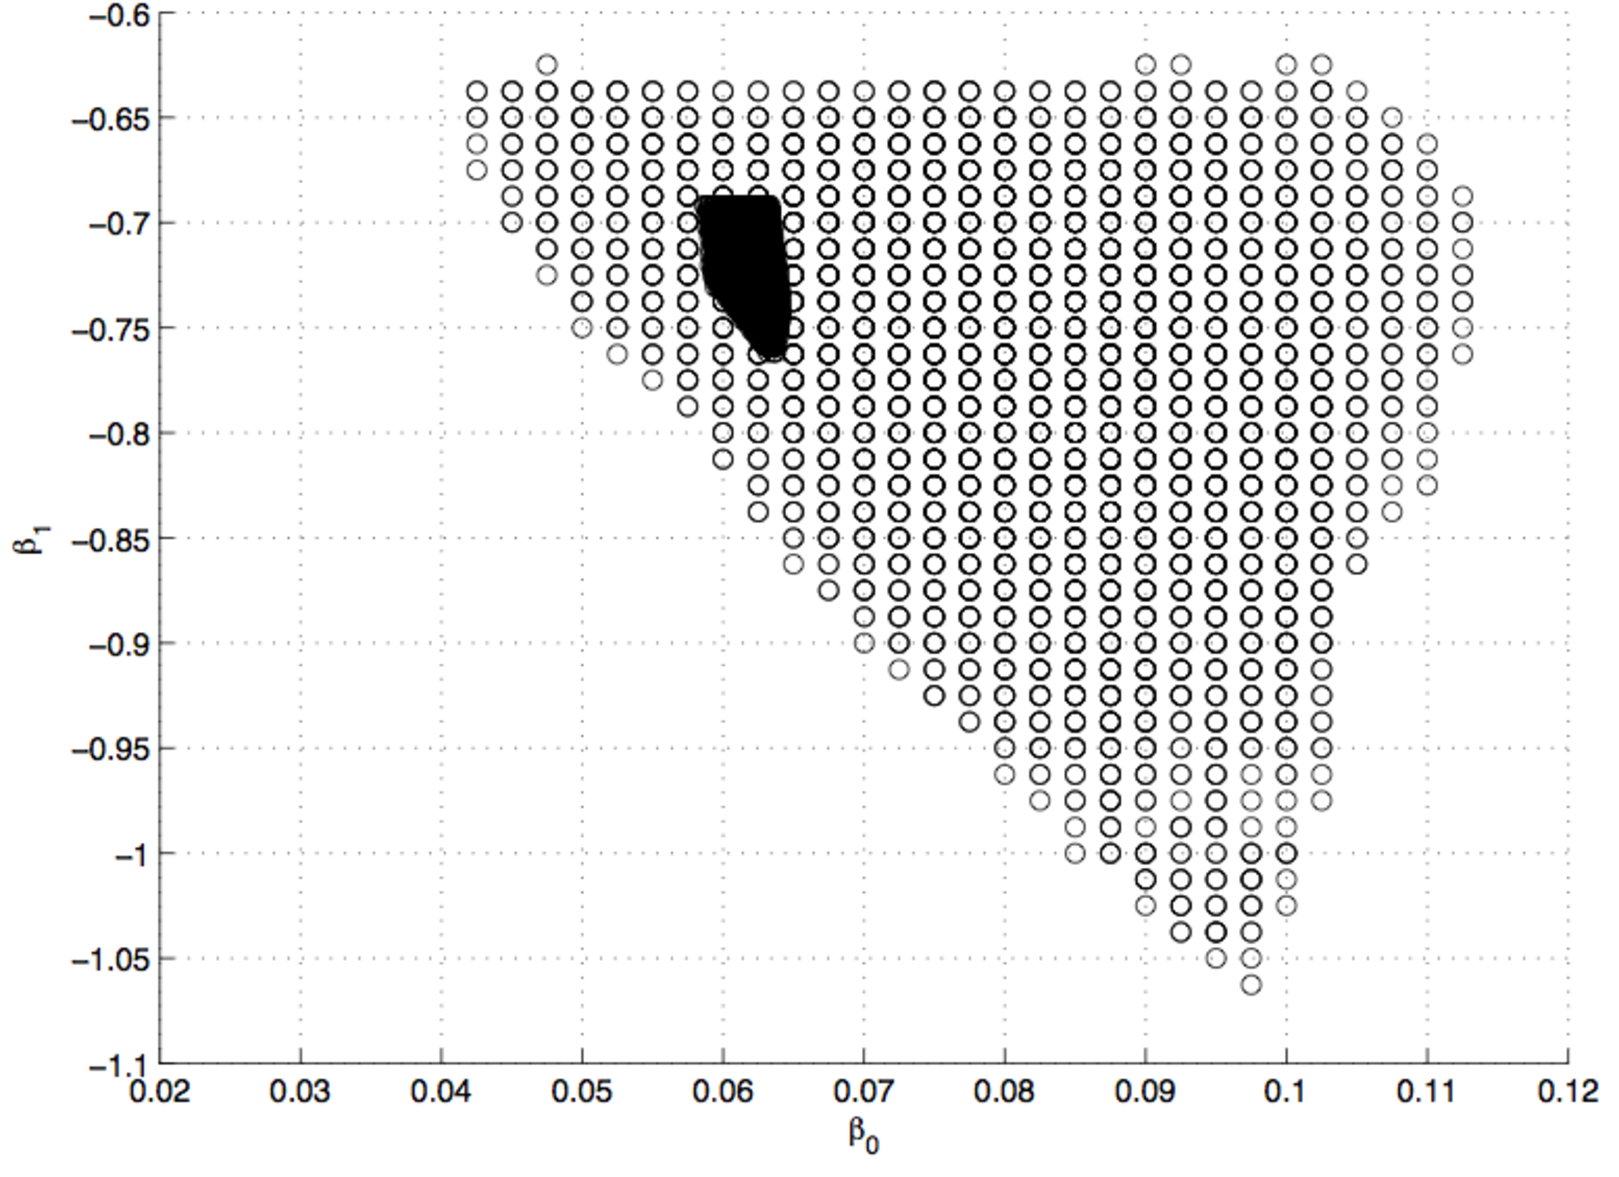
\includegraphics[width=3.6in,height=2.7in]{b0b1fig.pdf}
\end{figure}
\end{frame}
%-------------------------------------------------------------------------------
\begin{frame}
\frametitle{Identified Set and Confidence Set}

\begin{figure}
\centering
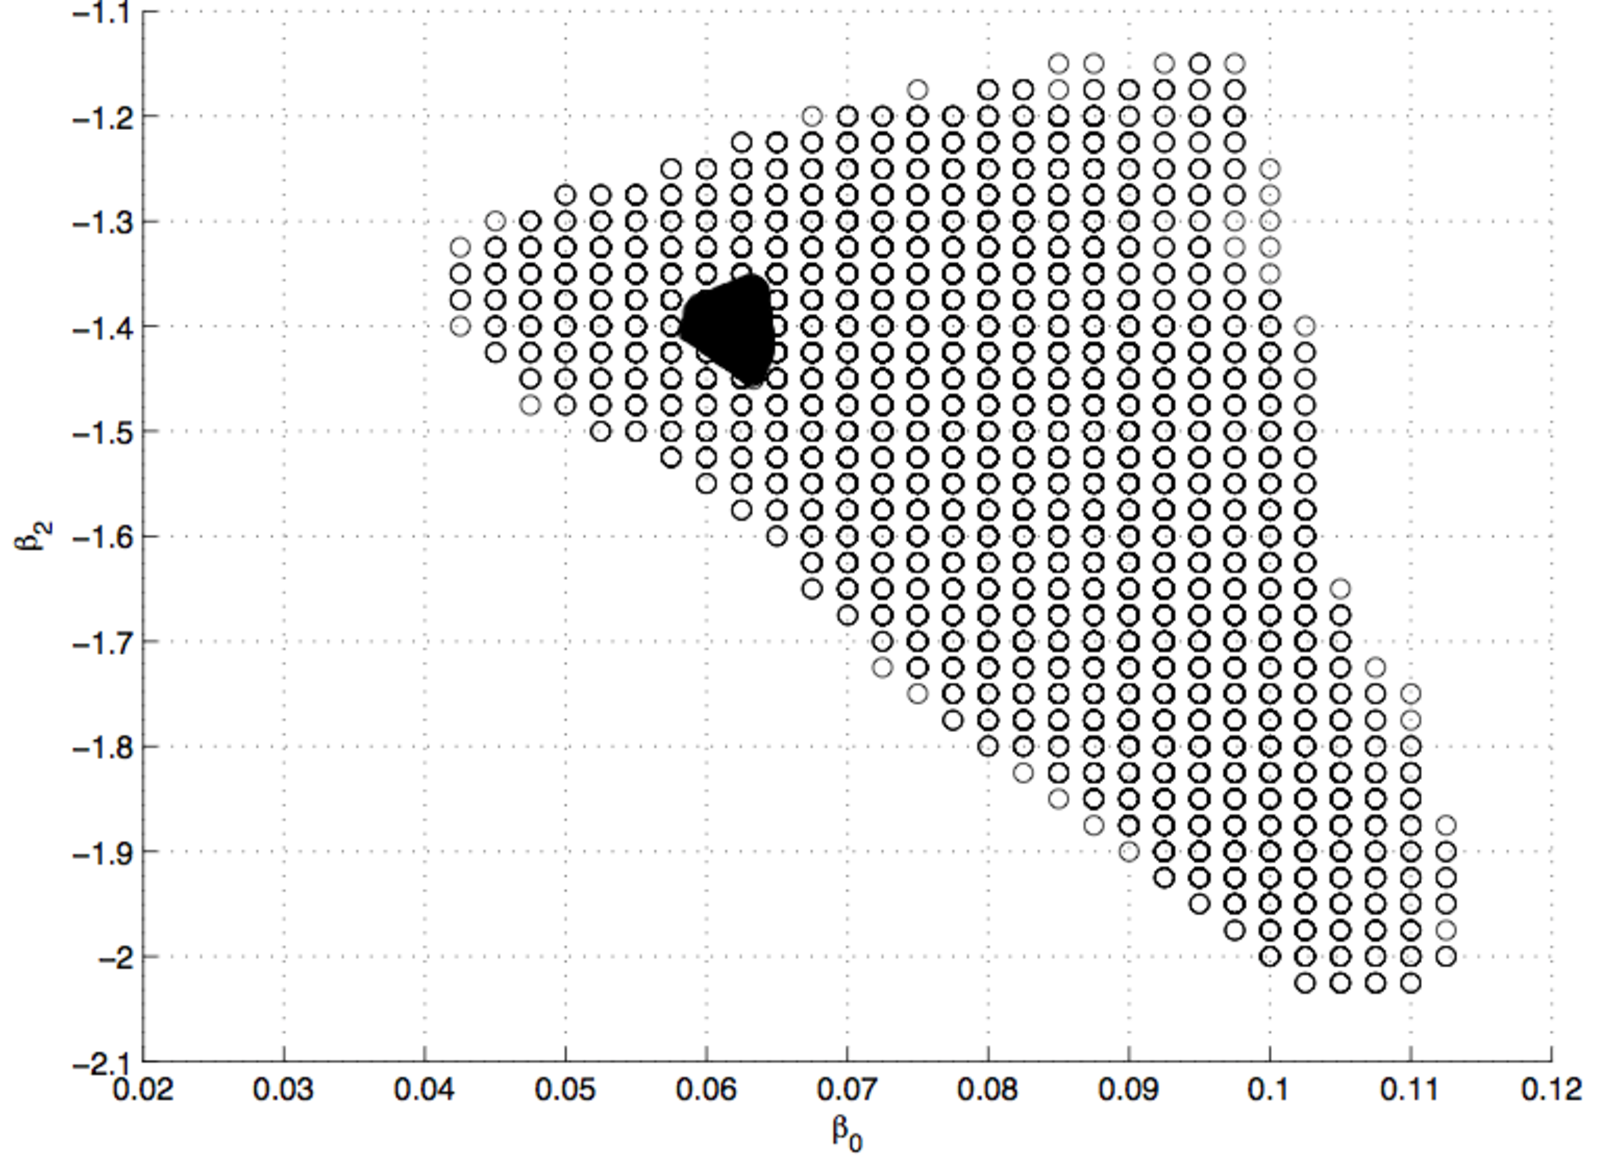
\includegraphics[width=3.6in,height=2.7in]{b0b2fig.pdf}
\end{figure}
\end{frame}
%-------------------------------------------------------------------------------
\begin{frame}
\frametitle{Identified Set and Confidence Set}

\begin{figure}
\centering
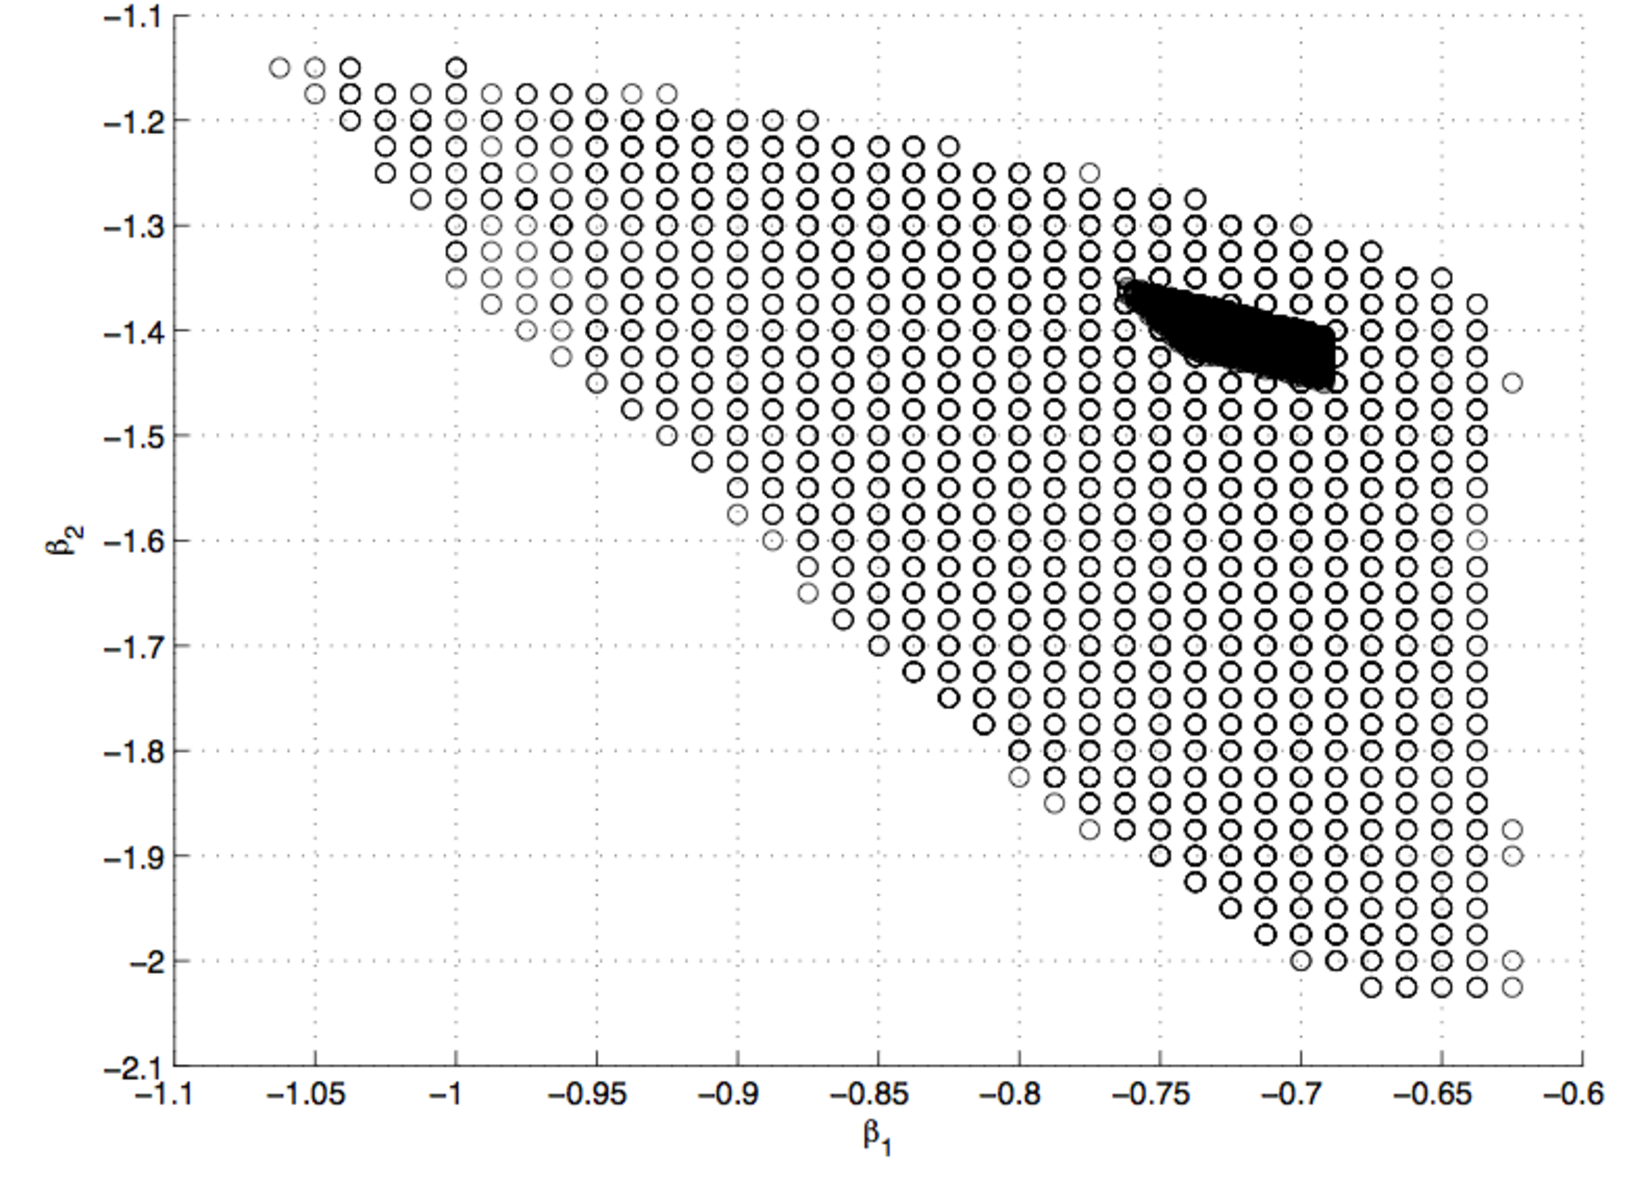
\includegraphics[width=3.6in,height=2.7in]{b1b2fig.pdf}
\end{figure}
\end{frame}
%-------------------------------------------------------------------------------
\begin{frame}
\frametitle{Empirical Application: $(r_{iht-1},R_{jt-1},dist_{j})\in\mathcal{J}_{ijt}$}

\begin{figure}[h]
\centering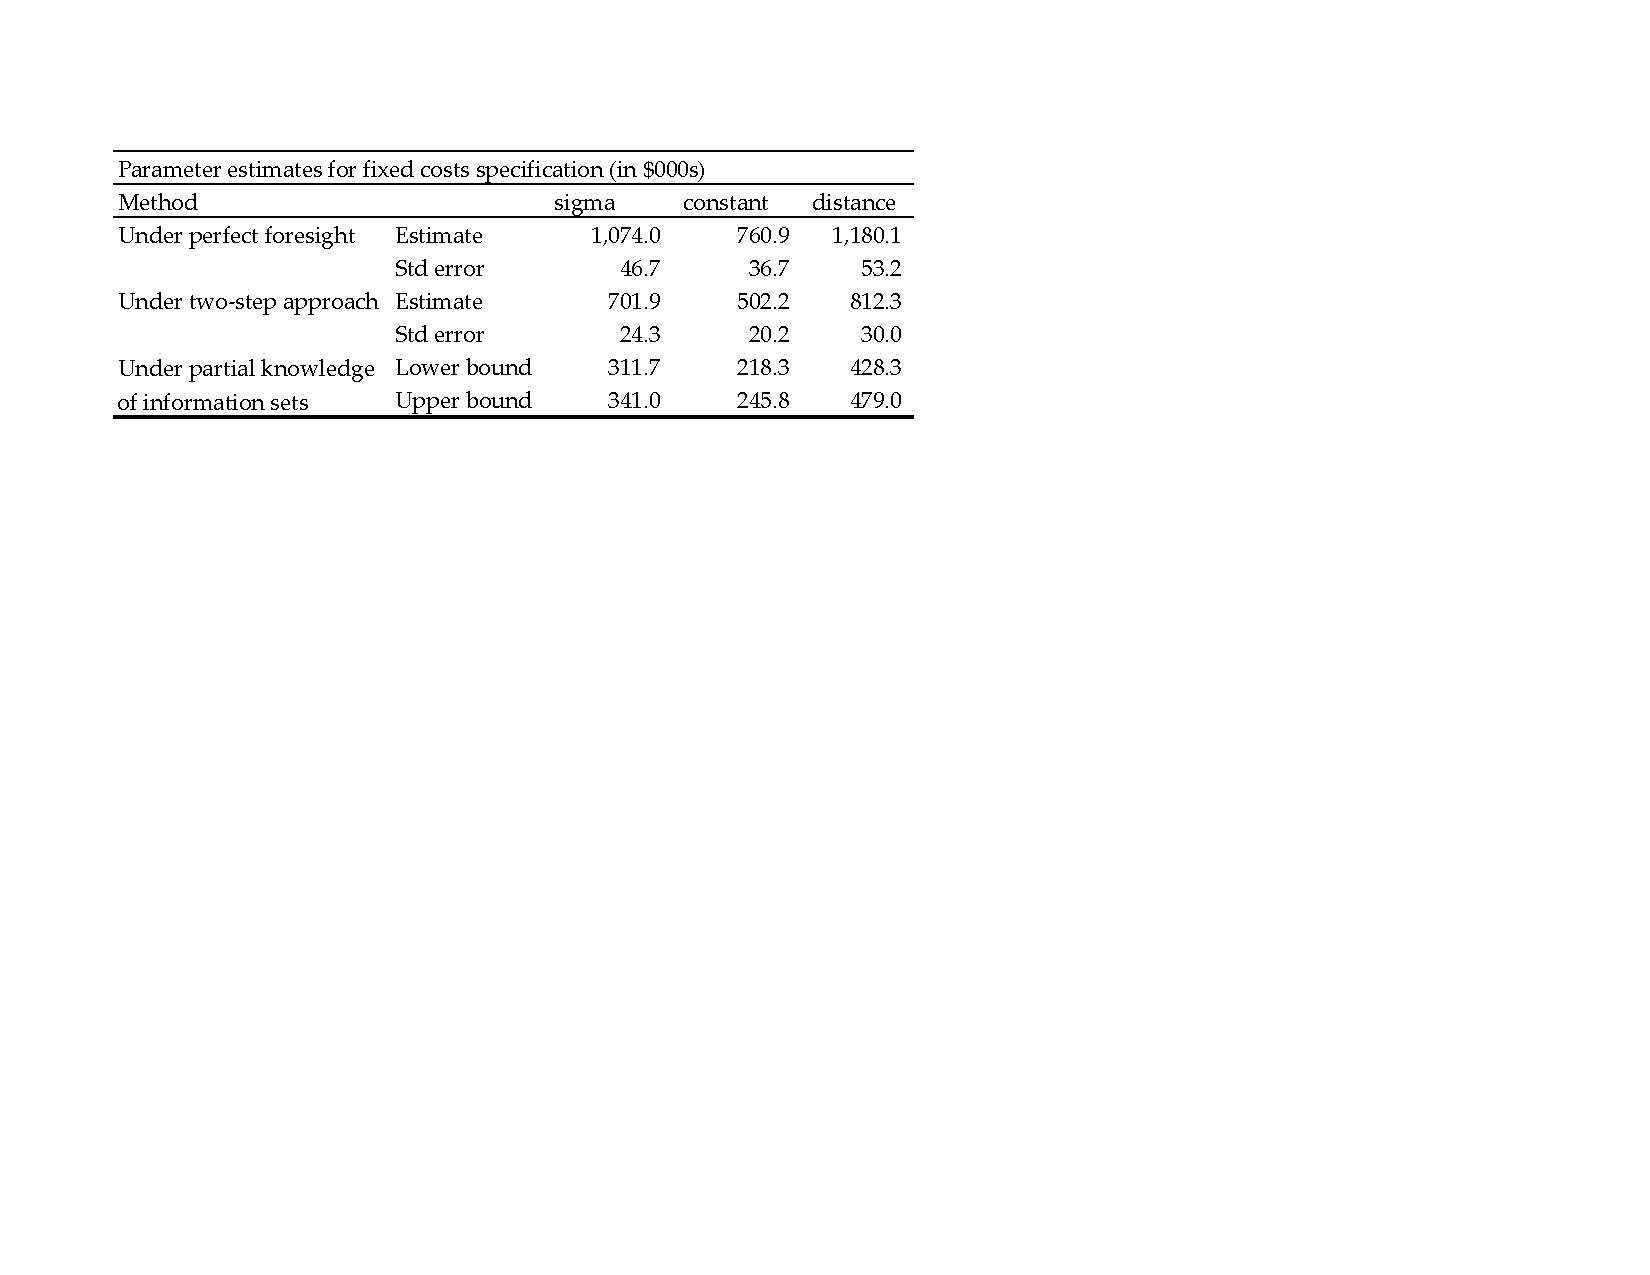
\includegraphics[width=1\linewidth]{parm_est_all.pdf}
\end{figure}

\end{frame}

%-------------------------------------------------------------------------------
\begin{frame}
\frametitle{Comparison of Different Methods.}

\begin{figure}[h]
\centering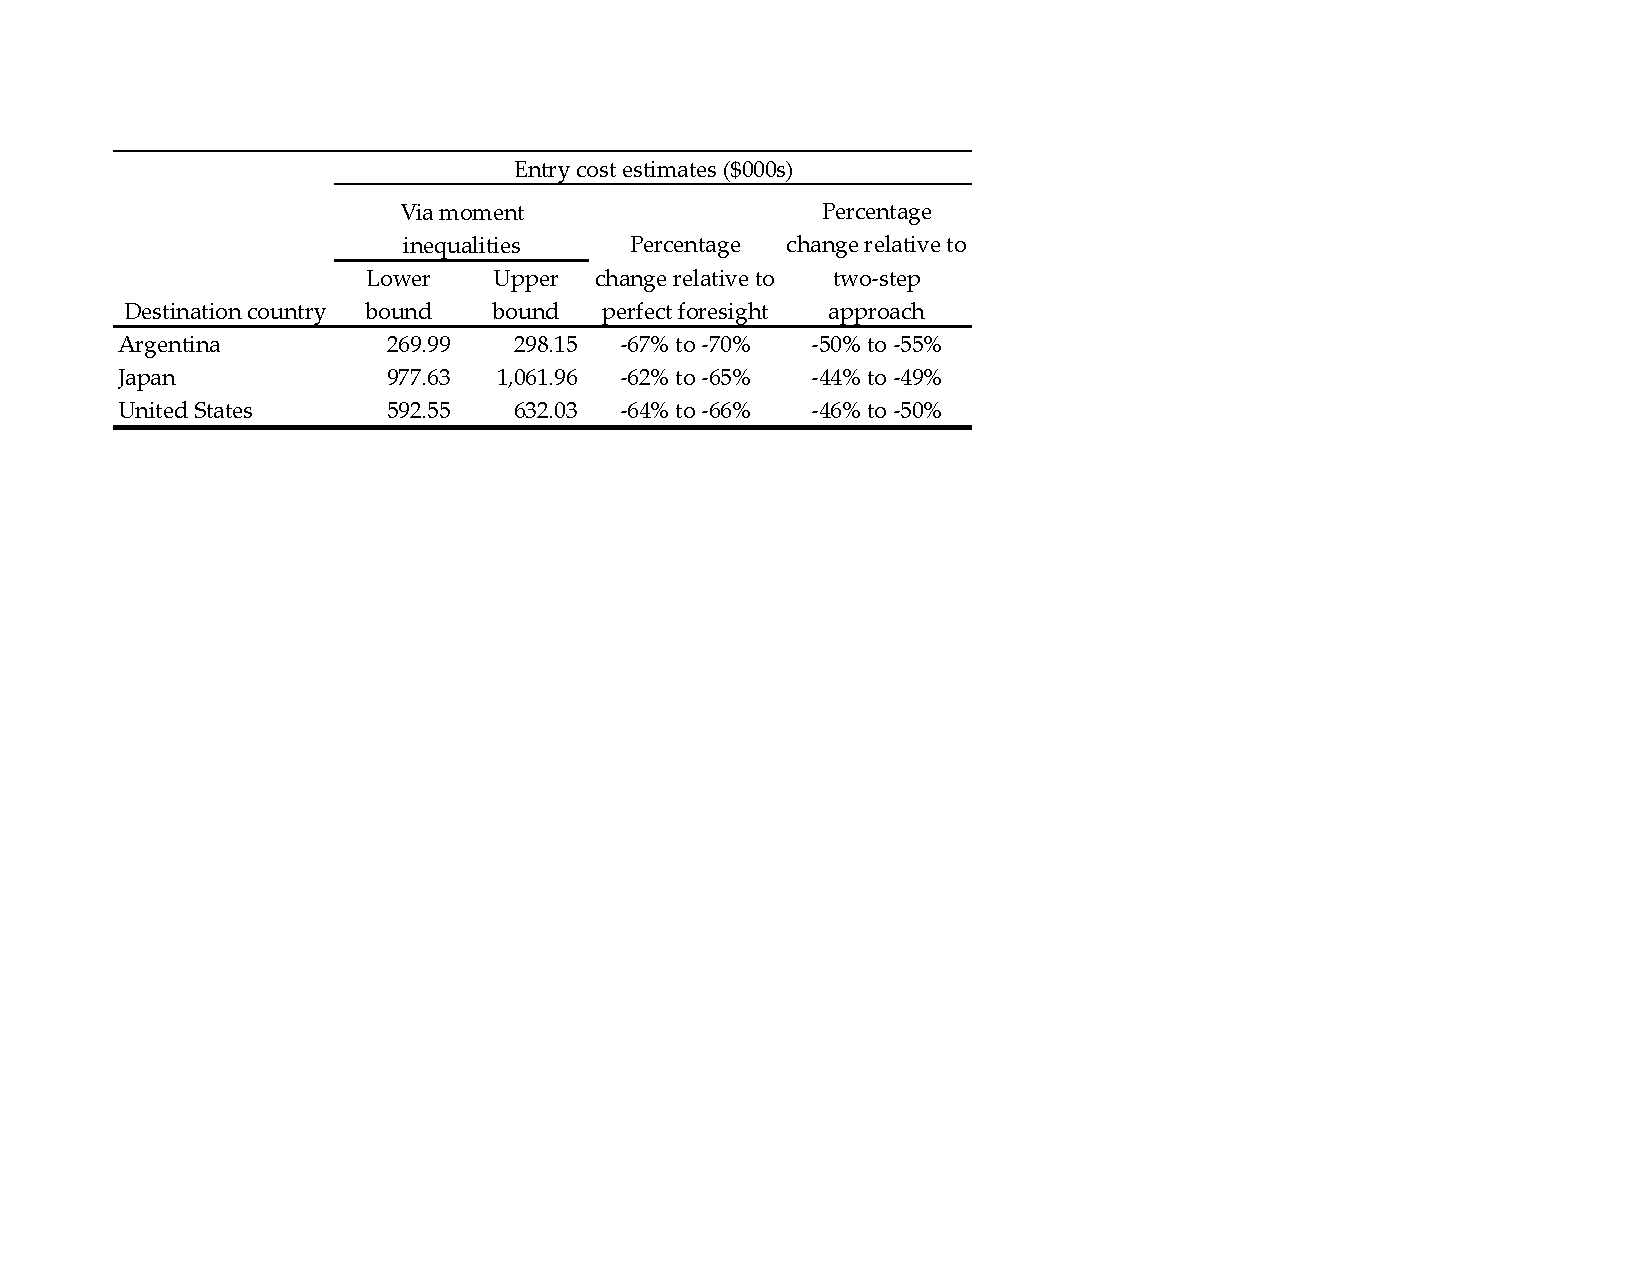
\includegraphics[width=1\linewidth]{entry_cost_compare}
\end{figure}

\end{frame}



\section{Inference}

%%%%%%%%%%%%%%%%%%%%%%%%

\begin{frame}
\centerline{ALTERNATIVE MOMENT INEQUALITIES ESTIMATORS:} %
\centerline{DEFINITION AND COMPUTATION}
\end{frame}

%%%%%%%%%%%%%%%%%%%%%%%%

\begin{frame}
\frametitle{Identified Set}

\begin{itemize}
\item Moment inequalities will generically lead to set identification. Given
a set $S$ of moment inequalities, the identified set is:  
\begin{equation*}
\Theta^{S}=\operatornamewithlimits{argmin}_{\theta}\sum_{s=1}^{S}\Big(\min%
\big\{0,\mathbbm{E}[m_{s}(Y,X,Z;\theta)]\big\}\Big)^{2}
\end{equation*}
\begin{figure}[h!]
\begin{center}
\subfigure{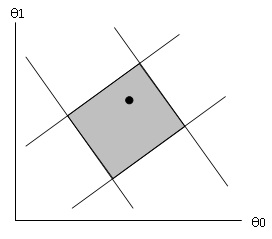
\includegraphics[scale=0.65]{Figure_1.jpg}}  \subfigure{%
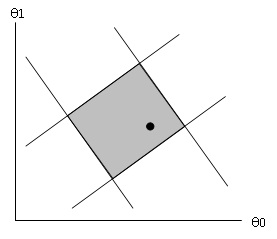
\includegraphics[scale=0.65]{Figure_2.jpg}} 
\end{center}
\end{figure}
\end{itemize}
\end{frame}

%%%%%%%%%%%%%%%%%%%%%%%%

\begin{frame}
\frametitle{Steps for Estimation}

\begin{itemize}
\item Step 1: Estimate the identified set given sample moments. 

\item Step 2: Perform inference on one or more of the following parameters: 

\begin{itemize}
\item Interval contained in the identified set: Pakes, Porter, Ho and Ishii
(Econometrica, 2014). 

\item Identified set: Chernozhukov, Hong and Tamer (Econometrica, 2007). 

\item True parameter vector: Andrews and Soares (Econometrica, 2010). 
\end{itemize}
\end{itemize}
\end{frame}

%%%%%%%%%%%%%%%%%%%%%%%%

\begin{frame}[label=estset] 
\frametitle{Estimation of the Identified Set}

\begin{itemize}
\item Estimation is based on the sample analogue of the moment inequalities:
\begin{equation*}
\overline{m}_{n,s}(\theta)=\frac{1}{n}\sum_{i=1}^{n}m_{s}(Y_{i},X_{i},Z_{i};%
\theta)
\end{equation*}
\begin{figure}[h!]
\begin{center}
\subfigure[Case 1]{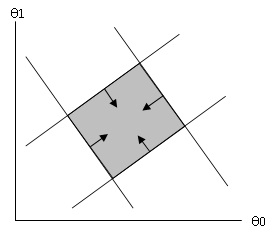
\includegraphics[scale=0.65]{Figure_3.jpg}}  %
\subfigure[Case 2]{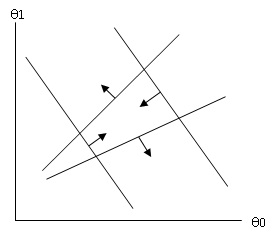
\includegraphics[scale=0.65]{Figure_4.jpg}} 
\end{center}
\end{figure}
\end{itemize}

\end{frame}

%%%%%%%%%%%%%%%%%%%%%%%%

\begin{frame}
\frametitle{Estimation of the identified set}

\begin{itemize}
\item Two possible criterion functions to define the estimated set: 

\begin{itemize}
\item Unweighted criterion function:  
\begin{equation*}
\hat{\Theta}^{S}_{n} = \operatornamewithlimits{argmin}_{\theta}\sum_{s=1}^{S}%
\Big(\min\{0,\overline{m}_{n,s}(\theta)\}\Big)^{2}
\end{equation*}

\item Weighted criterion function:  
\begin{equation*}
\hat{\Theta}^{S}_{n} = \operatornamewithlimits{argmin}_{\theta}\sum_{s=1}^{S}%
\Big(\min\{0,\Big[\frac{\overline{m}_{n,s}(\theta)}{\hat{\sigma}%
^{2}_{n,s}(\theta)}\Big]\}\Big)^{2},
\end{equation*}
with  
\begin{equation*}
\hat{\sigma}^{2}_{n,s}(\theta)=\frac{1}{n}%
\sum_{i=1}^{n}(m_{s}(Y_{i},X_{i},Z_{i};\theta)-\overline{m}%
_{n,s}(\theta))^{2}
\end{equation*}
\end{itemize}

\item The weighting lessens the influence of sample moments that have high
variance (likely to be further away from their population analogues).
\end{itemize}
\end{frame}

%%%%%%%%%%%%%%%%%%%%%%%%

\begin{frame}
\frametitle{Computation of the estimated set}

\begin{itemize}
\item We characterize the set $\hat{\Theta}^{S}_{n}$ by finding its
boundaries along any linear combination of the dimensions of vector $\theta$%
. 

\item If the moment functions $\{\overline{m}_{n,s}(\theta ): s=1,\dots,S\}$
are linear in $\theta$, use linear programming to find the extremum  
\begin{equation}
\begin{split}
& \max_{\theta}\quad f\cdot \theta \\
& \quad \text{s.t.} \\
& \quad \overline{m}_{n,s}(\theta )\geq 0,\text{ for }s=1,...,S.
\label{eq: optvert}
\end{split}%
\end{equation}

\item To find the maximum and minimum of our two-dimensional parameter $%
\theta$, we use:  
\begin{equation*}
f=\{[1,0],[-1,0],[0,1],[0,-1]\}.
\end{equation*}

\item Apply simplex routine in Matlab via \textit{linprog}
\end{itemize}
\end{frame}

%%%%%%%%%%%%%%%%%%%%%%%%

\begin{frame}
\frametitle{Computation of the estimated set}

\begin{itemize}
\item If there is no value of $\theta$ that verifies all the constraints, $%
\hat{\Theta}^{S}_{n}$ will be a singleton. 

\item This singleton is the outcome of a nonlinear optimization problem:  
\begin{equation*}
\hat{\Theta}^{S}_{n} = \operatornamewithlimits{argmin}_{\theta}\sum_{s=1}^{S}%
\Big(\min\{0,\Big[\frac{\overline{m}_{n,s}(\theta)}{\hat{\sigma}%
^{2}_{n,s}(\theta)}\Big]\}\Big)^{2}.
\end{equation*}

\item Use a nonlinear optimization package, like \textit{KNITRO} (in Matlab
via \textit{ktrlink} with license).
\end{itemize}
\end{frame}

%%%%%%%%%%%%%%%%%%%%%%%%

\begin{frame}
\frametitle{Computation of the estimated set: example}

\begin{itemize}
\item Sample moments:  
\begin{eqnarray*}
900-\theta _{0}(-2)-\theta _{1}(60) &\geq &0 \\
-900-\theta _{0}(2)-\theta _{1}(-55) &\geq &0 \\
200-\theta _{0}(1)-\theta _{1}(9) &\leq &0 \\
-200-\theta _{0}(-1)-\theta _{1}(-11) &\leq &0
\end{eqnarray*}
\end{itemize}
\end{frame}

%%%%%%%%%%%%%%%%%%%%%%%%%

\begin{frame}
\frametitle{Computation of the estimated set: example}

\begin{figure}[h!]
\begin{center}
\subfigure{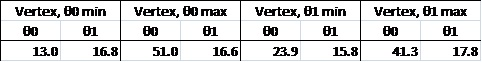
\includegraphics[scale=0.65]{Figure_5.jpg}} \subfigure{%
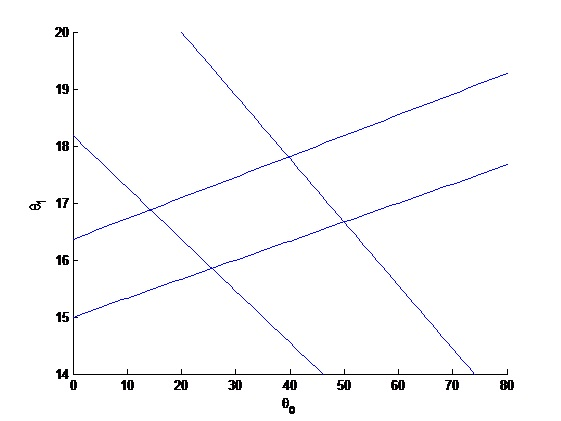
\includegraphics[scale=0.6]{Figure_6.jpg}}
\end{center}
\end{figure}
\end{frame}

%%%%%%%%%%%%%%%%%%%%%%%%%

\begin{frame}
\frametitle{Inference: General Intuition}

\begin{itemize}
\item Consider we want to test the null hypothesis: $H_{0}: \theta=\theta_{0}
$. 

\item We use the following statistic:  
\begin{equation*}
T_{n}(\theta_{0})=\sum_{s=1}^{S}\Big(\min\{0,\Big[\frac{\overline{m}%
_{n,s}(\theta_{0})}{\hat{\sigma}^{2}_{n,s}(\theta_{0})}\Big]\}\Big)^{2}.
\end{equation*}

\item The finite-sample null distribution of $T_{n}(\theta_{0})$ depends on
the degree of \textit{slackness} of the population moments--i.e. how much
greater than 0 is:  
\begin{equation*}
\mathbbm{E}[m_{s}(Y_{i},X_{i},Z_{i};\theta)],\quad\text{for $s=1,\dots,S$}.
\end{equation*}

\end{itemize}
\end{frame}

%%%%%%%%%%%%%%%%%%%%%%%%%

\begin{frame}
\frametitle{Inference: General Intuition}

\begin{itemize}
\item Key: need to infer whether a population moment binds at a particular
value $\theta_{0}$. 

\item Compute slackness factor, $SF_{n,s}(\theta_{0})$ 

\begin{itemize}
\item accounts for whether moment is likely to be binding 

\item moments likely to be nonbinding asymptotically --i.e. $\overline{m}%
_{n,s}(\theta)>>>0$--will have larger slackness factors 
\end{itemize}
\end{itemize}
\end{frame}

%%%%%%%%%%%%%%%%%%%%%%%%%

\begin{frame}
\frametitle{Inference: General Intuition}

\begin{itemize}
\item Three slackness factors proposed in the literature: 

\begin{itemize}
\item Assume that all the $S$ moments are binding at $\theta_{0}$: $%
SF_{I,s}=0$. 

\begin{itemize}
\item yields the most conservative test 
\end{itemize}

\item Moment Selection:  
\begin{equation*}
SF^{MS}_{n,s}(\theta_{0})=\mathbbm{1}\{\sqrt{n}(\frac{\overline{m}%
_{n,s}(\theta_{0})}{\hat{\sigma }_{n,s}(\theta_{0})})\leq\sqrt{2\ln (\ln (n))%
}\}
\end{equation*}

\item Shifted Mean: shift each moment proportionately to how far away from
binding it is in the sample.  
\begin{equation*}
SF^{SM}_{n,s}(\theta_{0})=(\frac{\overline{m}_{n,s}(\theta_{0})}{\hat{\sigma}%
_{n,s}(\theta_{0})})(\frac{1}{\sqrt{2\ln(\ln (n))}})\mathbbm{1}\{\frac{%
\overline{m}_{n,s}(\theta_{0})}{\hat{\sigma}_{n,s}(\theta_{0})}>0\}
\end{equation*}
\end{itemize}
\end{itemize}
\end{frame}

%%%%%%%%%%%%%%%%%%%%%%%%%

\begin{frame}
\frametitle{Inference for an Interval: PPHI (2011)}

\begin{itemize}
\item Objective: build confidence intervals for the vertices of the
estimated set, and use the outer bounds to form a unique confidence
interval. 

\item We need four elements for inference: 

\begin{itemize}
\item Vertices of the estimated set. 

\item Approximation to the asymptotic distribution of all the (weighted)
moments recentered at zero. 

\item Jacobian of the moments. 

\item Slackness factors. 
\end{itemize}
\end{itemize}

\end{frame}

%%%%%%%%%%%%%%%%%%%%%%%%%

\begin{frame}
\frametitle{Inference for an Interval}

\begin{itemize}
\item Approximation to asymptotic distribution of all the recentered
moments. 

\begin{itemize}
\item Draw $r=1,...,R$ times from a multivariate normal with zero mean, and 
covariance equal to the variance of the weighted moments 

\begin{itemize}
\item Take $R$ standard normal draws. 

\item Premultiply each draw by the Cholesky decomposition of the correlation
matrix evaluated at the vertex of interest, $\widehat{\Omega}_{n,S}(\hat{%
\theta})$:  
\begin{equation*}
\widehat{\Omega }_{n,S}(\hat{\theta})=diag(\widehat{\Sigma}_{n,S}(\hat{\theta%
}))^{-\frac{1}{2}}\widehat{\Sigma}_{n,S}(\hat{\theta})diag(\widehat{\Sigma}%
_{n,S}(\hat{\theta}))^{-\frac{1}{2}}.
\end{equation*}

\item Result:  
\begin{equation*}
q_{r}(\hat{\theta})=chol(\widehat{\Omega}_{n,S}(\hat{\theta}))N(0_{S},I_{S}).
\end{equation*}
\end{itemize}
\end{itemize}
\end{itemize}
\end{frame}

%%%%%%%%%%%%%%%%%%%%%%%%%

\begin{frame}
\frametitle{Inference for an Interval}

\begin{itemize}
\item Jacobian of the moments. 

\begin{itemize}
\item Compute the Jacobian of the sample unweighted moments, $\overline{m}%
_{n,s}(\theta)$, and evaluate the result at the vertex of interest: 

\item When the moments are linear in $\theta $, the derivative matrix
multiplied by $\theta $ simply equals the mean of the weighted moments:%
\begin{equation*}
\widehat{\Gamma }_{n,s}(\theta )\ast \theta =\frac{1}{n}\left[
\sum_{i=1}^{n}\frac{\Delta x_{i,s}}{\widehat{\sigma }_{n,s}(\theta )}%
,\sum_{i=1}^{n}\frac{\Delta y_{i,s}}{\widehat{\sigma }_{n,s}(\theta )%
}\right] \ast \binom{\theta _{0}}{\theta _{1}}=\frac{m_{n,s}(\theta )}{%
\widehat{\sigma }_{n,s}(\theta )}
\end{equation*}
\end{itemize}

\item evaluate the weights, $\widehat{\sigma }_{n,s}(\theta )$, at $\theta $
values equal to the relevant vertex.
\end{itemize}
\end{frame}

%%%%%%%%%%%%%%%%%%%%%%%%%

\begin{frame}
\frametitle{Inference for an Interval}

\begin{itemize}
\item Evaluate the slackness factor at the vertex of interest and normalize
by $\sqrt{n}$. 

\begin{itemize}
\item We could use either $SF_{n,s}^{MS}$ or $SF_{n,s}^{SM}$.\newline
The option described in Pakes, Porter, Ho, and Ishii (2011) is Shifted Mean: 
\begin{equation*}
SF_{n,s}^{SM}(\hat{\theta})\sqrt{n}=(\frac{\overline{m}_{n,s}(\hat{\theta})}{%
\hat{\sigma}_{n,s}(\hat{\theta})})(\frac{1}{\sqrt{2\ln (\ln (n))}})%
\mathbbm{1}\{\frac{\overline{m}_{n,s}(\hat{\theta})}{\hat{\sigma}_{n,s}(\hat{%
\theta})}>0\}\sqrt{n}
\end{equation*}
\end{itemize}
\end{itemize}
\end{frame}

%%%%%%%%%%%%%%%%%%%%%%%%%

\begin{frame}
\frametitle{Inference for an Interval}

\begin{itemize}
\item Compute the following linear programing problem for each draw $%
r=1,...,R$ and each vertex $\hat{\theta}$: (total of $2xdxR$ optimizations)  
\begin{equation}
\begin{split}
& \theta _{r}=\max_{\theta }\quad f\cdot \sqrt{n}(\hat{\theta}-\theta ) \\
& \quad \text{s.t.} \\
& \quad \widehat{\Gamma }_{n,S}(\hat{\theta})\sqrt{n}(\hat{\theta}-\theta
)+q_{r}(\hat{\theta})+SF_{n,S}^{SM}(\hat{\theta})\sqrt{n}\geq 0
\end{split}%
\end{equation}

\item As before, to find the maximum and minimum of our
two-dimensional parameter $\theta$, we use:  
\begin{equation*}
f=\{[1,0],[-1,0],[0,1],[0,-1]\}.
\end{equation*}
In equation (2), use the estimated
vertex $\hat{\theta}$ that corresponds to each vector $f$. 

\item We obtain $R$ draws of the asymptotic distribution of each of the
estimated vertices of the estimated set.
\end{itemize}
\end{frame}

%%%%%%%%%%%%%%%%%%%%%%%%%

\begin{frame}
\frametitle{Inference for an Interval}

\begin{itemize}
\item For each pair of vertices corresponding to a given dimension $d$ of $%
\theta$. 

\begin{itemize}
\item For the min vertex, take the $\alpha/2$ quantile of the set of
simulated vertices, $\theta_{r}$, $r=1,\dots,R$. Denote this number:  
\begin{equation*}
\underline{\theta}_{d,\alpha/2}.
\end{equation*}

\item For the max vertex, take the $(1-\alpha/2)$ quantile of the set of
simulated vertices, $\theta_{r}$, $r=1,\dots,R$  
\begin{equation*}
\overline{\theta}_{d,1-\alpha/2}.
\end{equation*}
\end{itemize}

\item The confidence interval for $\theta$ in the dimension $d$ with
significance level $\alpha$ is:  
\begin{equation*}
(\underline{\theta}_{d,\alpha/2},\overline{\theta}_{d,\alpha/2}).
\end{equation*}
\end{itemize}
\end{frame}

%%%%%%%%%%%%%%%%%%%%%%%%%

\begin{frame}
\frametitle{Set/Point Inference: General Intuition}

\begin{itemize}
\item Based on the inversion of an Anderson-Rubin T statistic. 

\item General steps in the algorithm: 

\begin{enumerate}
\item Define $\theta $ grids, $\widehat{\Theta }_{n}^{Grid}$ and $\widehat{%
\Theta }_{n}^{\epsilon }$, where $\widehat{\Theta }_{n}^{\epsilon }\subset 
\widehat{\Theta }_{n}^{Grid}$. 

\item Calculate $T_{r}(\theta )$, at a set of points in either $\widehat{%
\Theta }_{n}^{Grid}$ or $\widehat{\Theta }_{n}^{\epsilon }$ depending on
whether the focus of inference is the identified set or the true value of
the parameter. 

\item Determine a critical value as a quantile of $T_{r}(\theta)$ for $%
r=1,...,R$ 

\item Calculate $T^{obs}(\theta )$ at each $\theta \in \widehat{\Theta }%
_{n}^{Grid}$ with the observed data for all moments. 

\item Define the confidence set as those $\theta$ points where $%
T^{obs}(\theta)$ falls below the critical value. 
\end{enumerate}
\end{itemize}
\end{frame}

%%%%%%%%%%%%%%%%%%%%%%%%%

\begin{frame}
\frametitle{Forming the Grids: $\widehat{\Theta}_{I}^{Grid}$ and
$\widehat{\Theta}_{I}^{\epsilon}$}

$\widehat{\Theta }_{n}^{\epsilon }\subset \widehat{\Theta }_{n}^{Grid}$

\begin{figure}[h!]
\begin{center}
\subfigure{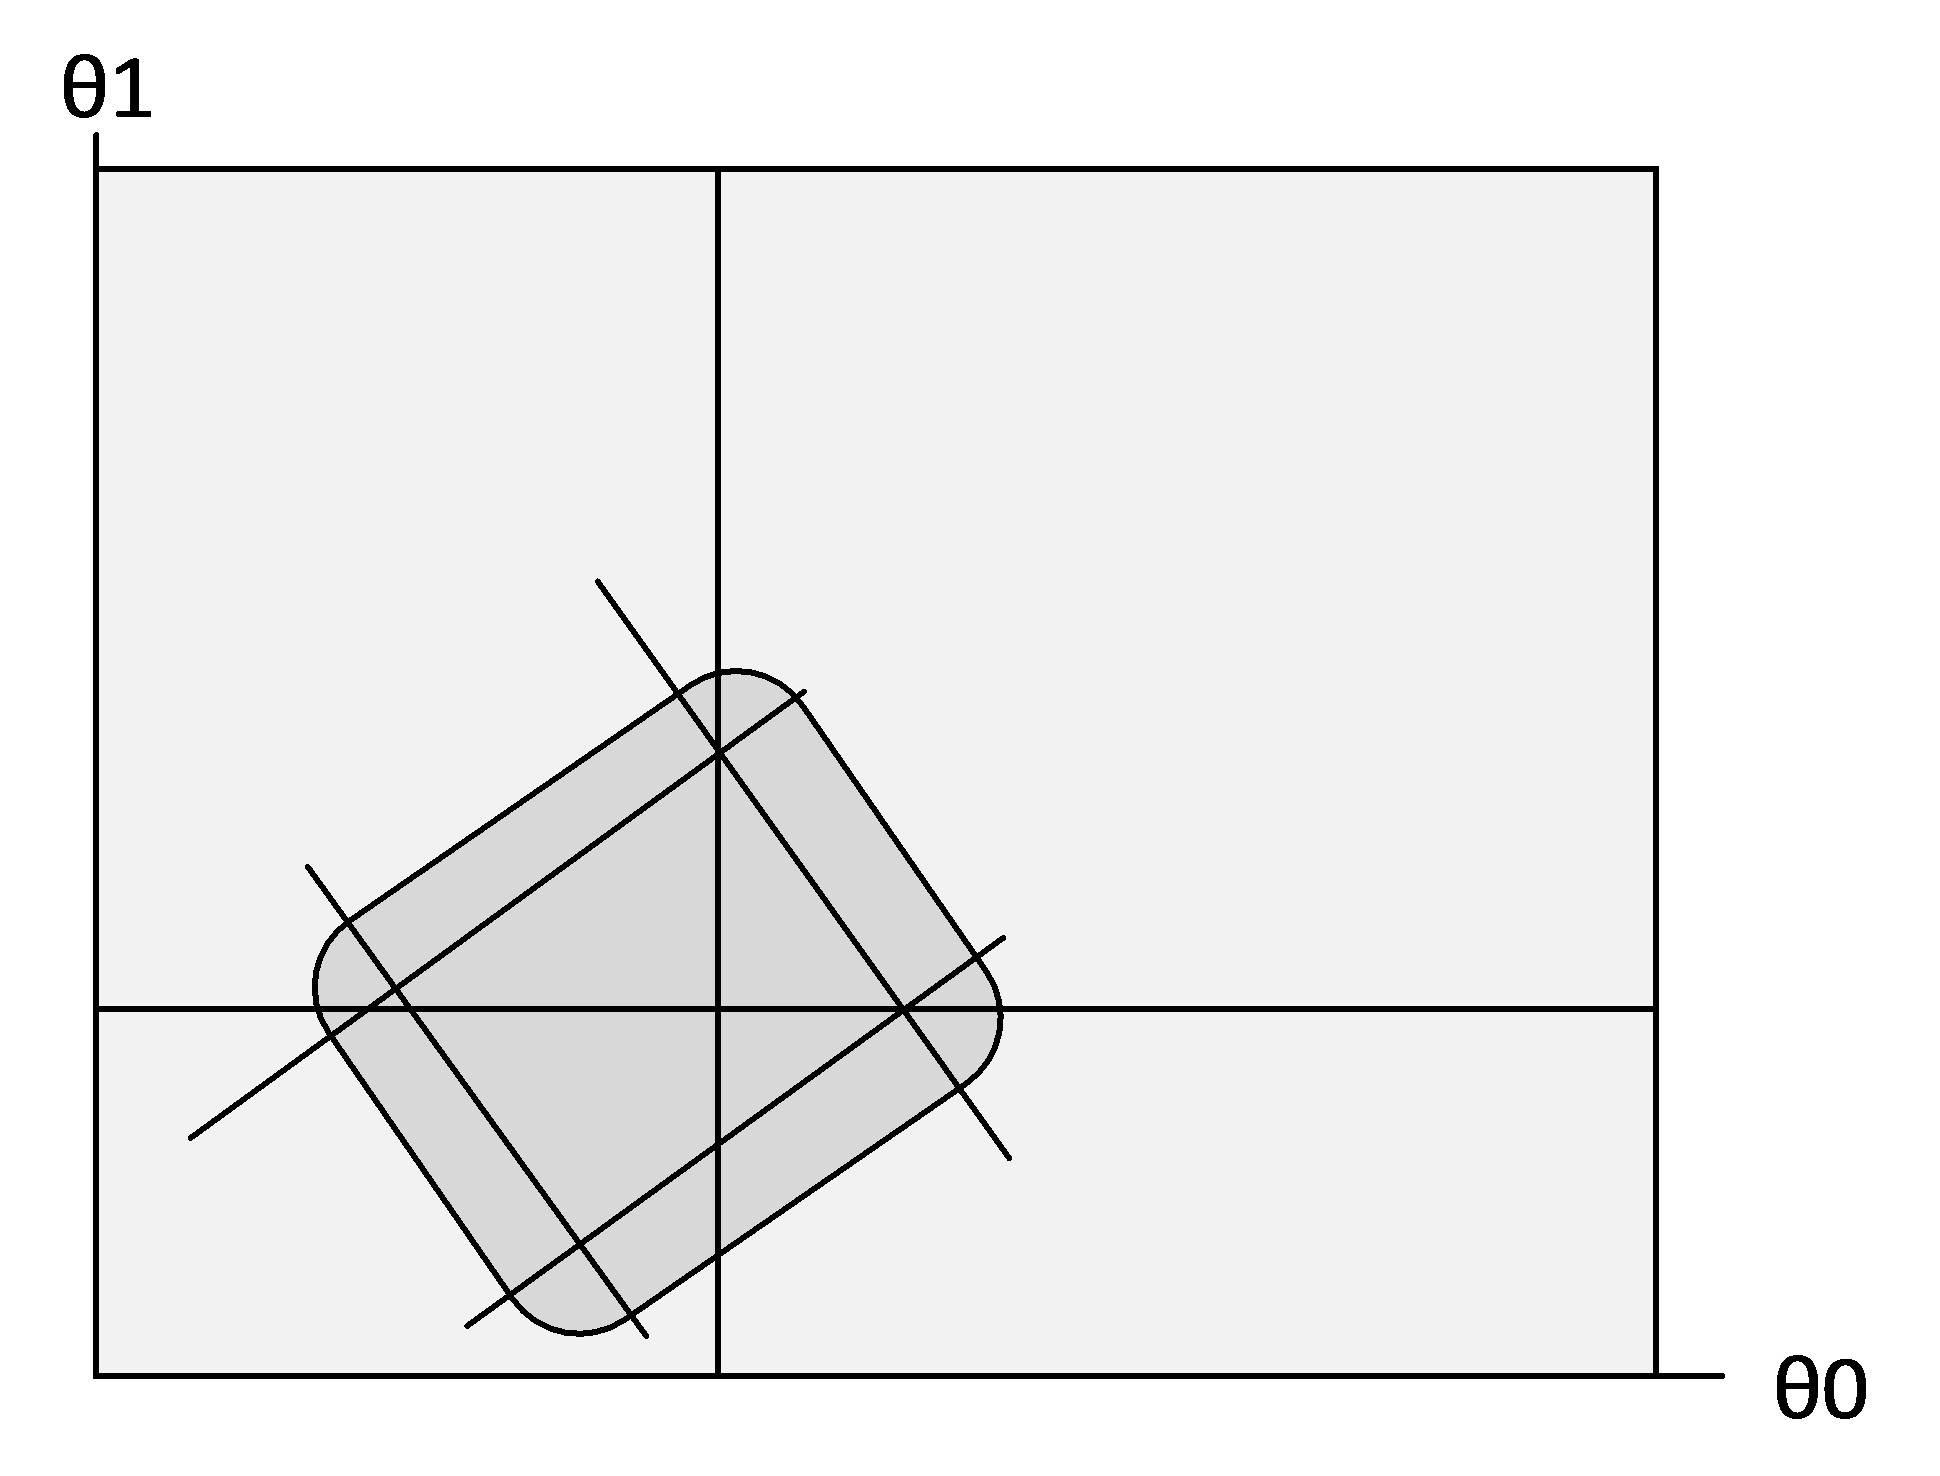
\includegraphics[scale=0.18]{Figure_9.jpg}}
\end{center}
\end{figure}
\end{frame}

%%%%%%%%%%%%%%%%%%%%%%%%%

\begin{frame}
\frametitle{Inference for the Identified Set}
\framesubtitle{Chernozhukov, Hong and Tamer (Econometrica,
2007)}
\begin{itemize}
\item Steps of the procedure: 

\begin{itemize}
\item (1) At $\theta \in \widehat{\Theta }_{n}^{\varepsilon }$, compute R
draws $\{q^{r}(\theta );r=1,\dots ,R\}$ such that: 
\begin{equation*}
q_{r}(\theta )=chol(\widehat{\Omega }_{n,S}(\theta ))N(0_{S},I_{S}),
\end{equation*}%
with 
\begin{equation*}
\widehat{\Omega }_{n,S}(\hat{\theta})=diag(\widehat{\Sigma }_{n,S}(\hat{%
\theta}))^{-\frac{1}{2}}\widehat{\Sigma }_{n,S}(\hat{\theta})diag(\widehat{%
\Sigma }_{n,S}(\hat{\theta}))^{-\frac{1}{2}}.
\end{equation*}%
Note that we are taking draws from the asymptotic distribution of the
normalized recentered moments, evaluated at each point $\theta $. 
\end{itemize}
\end{itemize}
\end{frame}

%%%%%%%%%%%%%%%%%%%%%%%%%

\begin{frame}
\frametitle{Inference for the Identified Set}

\begin{itemize}
\item Steps of the procedure (cont.) 

\begin{itemize}
\item (2) Compute one of the following T-statistic for each value of $\theta 
$ and draw $r$: 
\begin{equation*}
\begin{split}
T_{r}^{N}(\theta )& =\sum_{s=1}^{S}(\min \{0,q_{r,s}(\theta )\})^{2} \\
T_{r}^{MS}(\theta )& =\sum_{s=1}^{S}\{(\min \{0,q_{r,s}(\theta
)\})^{2}\times SF_{n,s}^{MS}(\theta )\} \\
T_{r}^{SM}(\theta )& =\sum_{s=1}^{S}(\min \{0,q_{r,s}(\theta
)+SF_{n,s}^{SM}(\theta )\})^{2}
\end{split}%
\end{equation*}

\item (3) For each draw $r$, take the maximum across $\theta $: 
\begin{equation*}
T_{r}^{\max }=\max_{\theta \in \widehat{\Theta }_{n}^{\varepsilon
}}T_{r}^{k}(\theta ),\quad k=\{N,MS,SM\}.
\end{equation*}
\end{itemize}
\end{itemize}
\end{frame}

%%%%%%%%%%%%%%%%%%%%%%%%%

\begin{frame}
\frametitle{Inference for the Identified Set}

\begin{itemize}
\item Steps of the procedure (cont.) 

\begin{itemize}
\item (4) Compute the critical value $c_{\alpha}$ as the $1-\alpha$ quantile
of the distribution of $\{T^{\max}_{r}; r=1,\dots,R\}$. 

\item (5) Return to the larger grid of theta points, $\widehat{\Theta }%
_{n}^{Grid}$, and calculate $T^{obs}(\theta )$ at each candidate value $%
\theta \in \widehat{\Theta }_{n}^{Grid}$: 
\begin{equation*}
T^{obs}(\theta )=\sum_{s=1}^{S}(\min \{0,\frac{\overline{m}_{n,s}(\theta )}{%
\hat{\sigma}_{n,s}(\theta )}\})^{2}
\end{equation*}

\item (6) Compare $T^{obs}(\theta)$ against $c_{\alpha}$ and accept $\theta$
into the confidence set whenever $T^{obs}(\theta)$ $<$ $c_{\alpha}$. 
\end{itemize}
\end{itemize}
\end{frame}

%%%%%%%%%%%%%%%%%%%%%%%%%

\begin{frame}
\frametitle{Inference for the Identified Set: Example}

\begin{figure}[h!]
\begin{center}
\subfigure{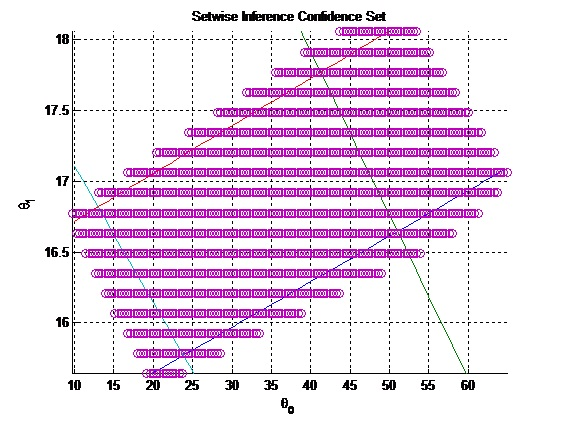
\includegraphics[scale=0.65]{Figure_10.jpg}}
\end{center}
\end{figure}
\end{frame}

%%%%%%%%%%%%%%%%%%%%%%%%%

\begin{frame}
\frametitle{Inference for the True Parameter}
\framesubtitle{Andrews and Soares (2010)}

\begin{itemize}
\item Steps of the procedure: 

\begin{itemize}
\item (1) At every $\theta \in \widehat{\Theta }_{n}^{Grid}$, calculate $%
\{q_{r}(\theta );$ $r=1,\dots ,R\}$: 
\begin{equation*}
q_{r}(\theta )=chol(\widehat{\Omega }_{n,S}(\theta ))N(0_{S},I_{S})
\end{equation*}

\item (2) For each of these $\theta $ and $r$, calculate: $T_{r}(\theta )$, $%
T_{r}^{MS}(\theta )$, or $T_{r}^{SM}(\theta )$. 

\item (3) For each $\theta $, calculate the $(1-\alpha )$ quantile. This the
critical value, $c(\alpha ,\theta )$. 

\item (4) Calculate $T^{obs}(\theta )$ at each candidate value $\theta \in 
\widehat{\Theta }_{n}^{Grid}$. 

\item (5) Compare $T^{obs}(\theta )$ against $c(\alpha ,\theta )$ and accept 
$\theta $ into the confidence set whenever $T^{obs}(\theta )$ $<$ $c(\alpha
,\theta )$. 
\end{itemize}
\end{itemize}
\end{frame}


\end{document}
